\subsection{Generating the resource graph}
\label{sec:gener-reso-graph}

The resource graph represents the cluster of compute nodes on which
the task graph will be executed. The resource graph is generated
by assuming the capabilities lie in a fixed range. In generating
them synthetically we avoid being biased by a single architecture and
we can evaluate our system for different characteristics. The process
of generating the synthetic resource graph is described below:

\begin{itemize}

\item The compute nodes are assumed to belong under two categories of
processing units, mainly CPUs and GPUs. The scalar instructions of a
Processing Element (\textbf{PE}) that represents a CPU is much higher
that that of a GPU. At the same time parallel vector operations that a
\textbf{PE} representing a GPU is much higher compared to that of a
CPU. Using this we define a range from which we assign the respective
\textbf{PE}'s capabilities.

\item The network system that interconnects these PEs are considered
to be a two dimensional mesh. In this topology the PEs are connected
in a grid with communication links between them. The 2D Mesh is one of
most commonly found network interconnects in HPC clusters. The
bandwidths are considered to be varying in nature, so each of the
link's bandwidth is chosen from a distribution.

\end{itemize}

The resource graph that is generated is truly hetrogeneous both
computations and communciation. A sample resource graph is shown in
fig \ref{fig:res} at level 0, as part of our clustering approach.
Mapping the task graph on to such a hetrogeneous is NP hard. The
problem mainly lies in the size of the resouce graph and the number of
ways in which the task graph can be mapped on to the resource graph.

In our approach we apply a set of heuristics to tackle the problem in
several phases. The various stages this is performed in shown here:

\begin{itemize}

\item Firstly, we form virtual representations of the resource graph by
clustering the nodes. This is done in such a way that we balance the
capabilities of the virtual nodes formed, minimizing the
communication volume.

\item Secondly, instead of doing this in a single stage, we construct
this in several stages by clustering half the nodes from the previous
stage. We end up with a structure consisting of several levels, where
the $ Number\ of\ levels = log_2 ( Number\ of\ Nodes )$.

\item The communication bandwidth between the clustered nodes is
determined by,\\ ${ \sum ( \min for same destn ( \max bw R^i, R^j ) )
) }$\\ The max bandiwdths between any ${R^i}$ is determined by floyd
warshall algorithm.

\item The capabity of each of the PEs that are clustered together are
aggregated to form the larger node.

\item In each level PEs with high communication bandwidth and balanced
capabilities are clustered together. In doing this in a bottom up
approach i.e. clustering instead of partitioning, we allow the nodes to
form without ignoring communication links between the nodes. This also
avoids the formation of dangling nodes in the graph.

\end{itemize}

\begin{figure}[ht]
  % \centering
  \includegraphics[scale=0.43]{./figures/resource}
  \caption{Clustering of a resource graph}
  \label{fig:res}
\end{figure}

In fig \ref{fig:res} we show our clustering approach on a 4x2 mesh. At
each level suitable nodes are clustered together to form a larger node.

\subsection{Application partitioning}
\label{sec:appl-part}
